\section{Convolution} 
\label{sec:convolution}
In \ref{sec:signals_and_systems} wurde gezeigt, dass Lineare Zeit-invariante Systeme sich vollständig durch ihre Impulsantwort
charakterisieren lassen. Hier werden Impulsantwort und die Convolution-Summe definiert.

\cite[S. 11]{oppenheim1999} formuliert zur Präzisierung der in \ref{sec:signals_and_systems} gezeigten Interpretation eines Signals als Summe skalierter und verzögerter Einheitsimpulse eine allgemeine Summenformel, mit der eine beliebige Folge $x[n]$ ausgedrückt wird:
\begin{equation}
    x[n]=\sum_{k=-\infty}^\infty x[k]\delta[n-k]
    \label{eq:scaled_unit_sum}
\end{equation}
Die mathematische Beschreibung der diskreten Convolution wird daraus wie folgt abgeleitet: 

Sei $y[n]$ das Ausgangssignal eines LTI-Systems, resultierend aus einem Eingangssignal $x[n]$. Sei $h_k[n]$ die Antwort eines Systems
auf einen Einheitsimpuls an Index $n=k$. Es gilt:

\begin{equation}
    y[n]=T\left( \sum_{k=-\infty}^{\infty}x[k]\delta[n-k] \right).
\end{equation}

Nach Superposition (Linearität) gilt auch:

\begin{equation}
    y[n]=\sum_{k=-\infty}^{\infty}x[k]T(\delta[n-k])=\sum_{k=-\infty}^{\infty}x[k]h_k[n].
    \label{eq:timevariant_equation}
\end{equation}
In Gleichung \ref{eq:timevariant_equation} ist $h_k[n]$ vom Laufindex der Summenfunktion abhängig. Es würden für die Berechnung der Summe also
genauso viele System-Antworten benötigt, wie Summierungen ausgeführt werden.
Unter Forderung der Zeitinvarianz des Systems fällt diese Eigenschaft weg:

\begin{equation}
    y[n]=\sum_{k=-\infty}^{\infty}x[k]h[n-k].
    \label{eq:convolution_sum}
\end{equation}
Die Gleichung \ref{eq:convolution_sum} wird als \textit{Convolution-Summe} bezeichnet \cite[S. 22f]{oppenheim1999}. Als kürzere Schreibweise für 
die Convolution zweier Signale $x$ und $h$ zu einem Ausgangssignal $y$ dient die Schreibweise $y[n]=x[n]*h[n]$.

Das Prinzip kann anhand eines simplen Anwendungsfalls, dem Tiefpassfilter, versanschaulicht werden.
Visualisierungen in diesem Abschnitt sind an die Grafiken von Richard Lyons \cite[Kap. 5]{lyons2011} angelehnt.
Tiefpassfilter können in der diskreten Zeitdomäne durch ein von \cite[S. 220]{lyons2011} \textit{Moving Average Filter} genanntes System realisiert werden.
Für jedes Sample $y[n]$ des Ausgangssignals wird ein Mittelwert der Eingangs-Samples $x[n-k]$ bis $x[n]$, $k\in\mathbb{N}$, gebildet.
Tiefpassfilter dämpfen die höheren Frequenzen des Spektrums eines Signals. Moving Average Filter erzielen diesen Effekt
durch stärkere Glättung schnellerer (höherfrequenter) Veränderungen in den gemittelten Werten im Vergleich zu langsameren (niedrigfrequenter) Veränderungen.
Bei einer Berechnung des Mittelwerts von 5 Samples gilt
\begin{equation}
    y[n]=\frac{1}{5}\sum_{k=0}^4x[n-k]\iff y[n]=\sum_{k=0}^4\frac{1}{5}x[n-k].
    \label{eq:mov_avg_filter}
\end{equation}
\cite[S. 172]{lyons2011}.

Die Summenformel zur Berechnung der Ausgangs-Samples dieses Moving Average Filters \ref{eq:mov_avg_filter} ähnelt der Convolution-Summe \ref{eq:convolution_sum}.
Auffällige Unterschiede sind endliche Summierung und Verwendung eines festen Koeffizienten pro Summand.
Der für jeden Summanden verwendete Koeffizient $\frac{1}{5}$ kann als diskretes Signal, bestehend aus 5 Samples, mit den Werten $\frac{1}{5}$ interpretiert werden:
\begin{equation}
    \label{eq:fir_convsum}
    y[n]=\sum_{k=0}^4h[k]x[n-k]\text{ mit }h=\left(\frac{1}{5},\,\frac{1}{5},\,\frac{1}{5},\,\frac{1}{5},\,\frac{1}{5}\right).
\end{equation} \cite[S. 172 f]{lyons2011}.

Die Summenformel \ref{eq:fir_convsum} ist eine endliche Convolution-Summe mit vertauschter Indizierung von Eingangs-Signal und Impulsantwort. Nach der
kommutativen Eigenschaft der Convolution ist \ref{eq:fir_convsum} äquivalent zu \ref{eq:convolution_sum} \cite[Kap. 2]{oppenheim1999}. So konstruierte Filter werden \textit{Finite Impulse Response Filter},
kurz \textit{FIR-Filter}, genannt. Die Filterkoeffizienten der Mittelwertberechnung bilden, wie die Notation als $h$ impliziert, die Impulsantwort einses Systems: eines
Moving Average Filters. Aus Anwendung dieses konstruierten FIR-Filters auf einen Einheitspimpuls resultiert das diskrete Signal $h$ aus Gleichung \ref{eq:fir_convsum}.
Die Wirkung des Moving Average Filters wird durch plotten von Ein- und Ausgangssignal anschaulich:

\begin{figure}[H]
    \centering
    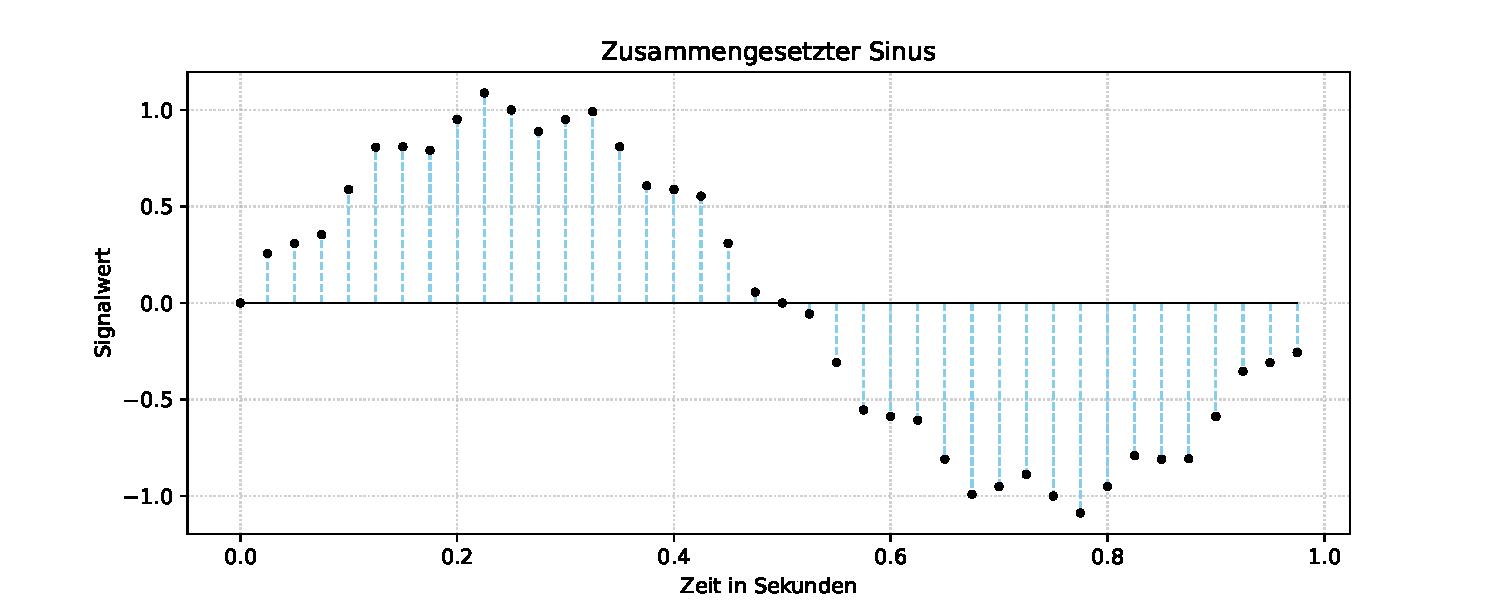
\includegraphics[width=0.5\textwidth]{graphic/python/chapter3/compound_sinusoid.pdf}
    \caption{Ein diskretes Signal, zusammengesetzt aus Sinusschwingungen mit den Frequenzen $f_0=1\,\text{Hz}$, $f_1=10\,\text{Hz}$, und $f_2=20\,\text{Hz}$}
    \label{fig:comp_sinusoid}
\end{figure}

Die Anwendung des Moving Averager Filters resultiert in einer deutlichen Glättung des Signals, aber auch zu einer zeitlichen Verzögerung des Signals:

\begin{figure}[H]
    \centering
    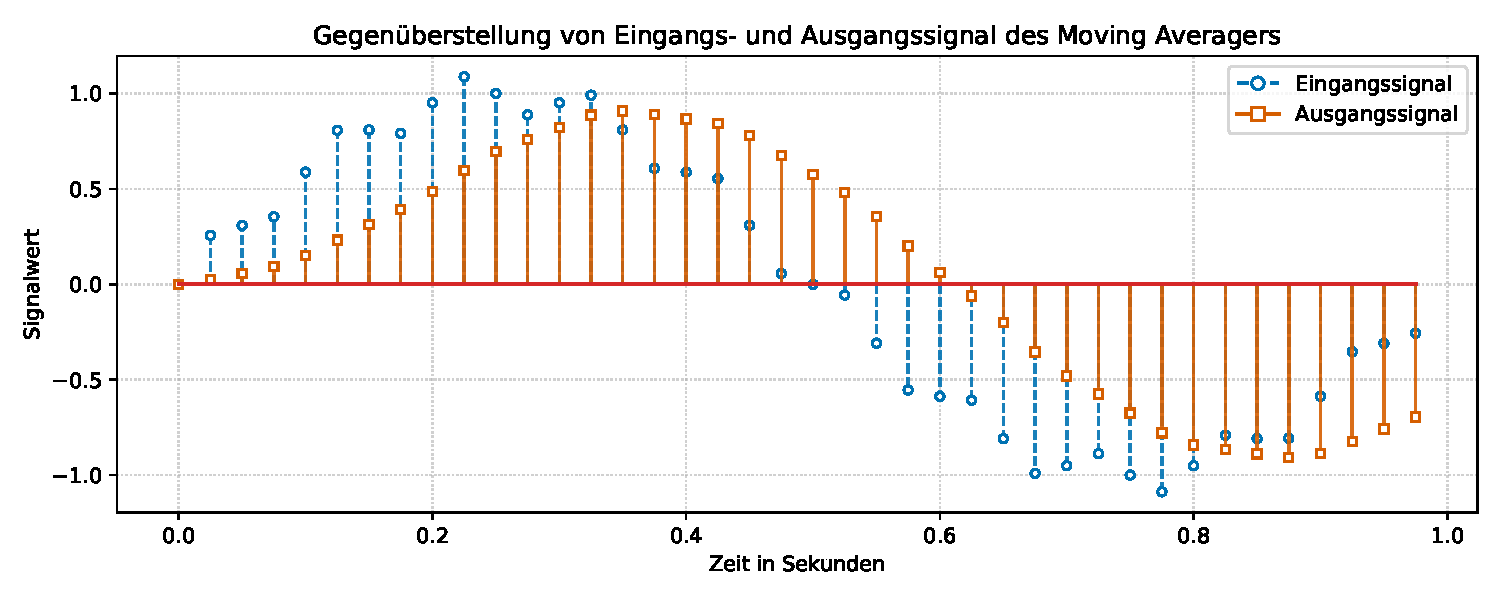
\includegraphics[width=0.5\textwidth]{graphic/python/chapter3/comparison_compound_filtered.pdf}
    \caption{Das gefilterte Signal, über das ungefilterte Signal aus Abbildung \ref{fig:comp_sinusoid} vorgeblendet}
    \label{fig:in_out_comparison}
\end{figure}

Dieser FIR-Filter ist ein anschauliches Beispiel für den Prozess der Convolution. 
Die Convolution-Summe selbst ist in allen Anwedungen von Convolution in der Signalverarbeitung gleich. In echten 
Anwendungsfällen werden oft weit längere Impulsantworten und Signale verwendet. Das resultiert in weit mehr Summanden und Multiplikationen
pro berechnetem Ausgangs-Sample. Besonders in Echtzeitanwendungen, in denen eine hinreichend schnelle Berechnung der Ausgangssamples nötig ist, führt die direkte Berechnung von Convolution-Summen zu
untragbaren Laufzeiten. Bei der häufigen Audio-Abtastrate von 44,1kHz bleiben für
die Berechnung eines Blockes von 256 Ausgangs-Samples weniger als 6 Millisekunden. Für die praktische Anwendung von Convolution zur Abbildung von Systemen wird eine Lösung mit besserem Laufzeitverhalten genutzt.
Diese basiert auf dem Convolution-Theorem.

\subsection{Das Convolution-Theorem}
\label{sec:convolution_theorem}
Seien $X(e^{i\omega})$, $H(e^{i\omega})$ und $Y(e^{i\omega})$ die diskreten Fourier-Transformationen des Eingangssignals $x$, der Impulsantwort $h$, und 
des Ausgangssignals $y$ einer Convolution $y[n]=x[n]*h[n]$. Dann gilt:

\begin{equation}
    \label{eq:convolution_theorem}
    Y(e^{i\omega})=X(e^{i\omega})\cdot H(e^{i\omega}).
\end{equation} 
Die Convolution zweier Signale in der Zeitdomäne ist äquivalent zu einer Multiplikation der Signale in der Frequenzdomäne. Mit einer inversen diskreten Fourier-Transformation
des Ausgangs-Spektrums $Y(e^{i\omega})$ wird das Ausgangssignal in die Zeitdomäne übertragen \cite[Kap.2]{oppenheim1999}. 
Bei hinreichend effizienter Berechnung der (inversen) diskreten Fourier-Transformationen kann somit die direkte Berechnung der Convolution-Summe vermieden und durch Multiplikation in der Frequenzdomäne ersetzt werden.